% see http://info.semprag.org/basics for a full description of this template
\documentclass[cm,linguex]{glossa}

% possible options:
% [times] for Times font (default if no option is chosen)
% [cm] for Computer Modern font
% [lucida] for Lucida font (not freely available)
% [brill] open type font, freely downloadable for non-commercial use from http://www.brill.com/about/brill-fonts; requires xetex
% [charis] for CharisSIL font, freely downloadable from http://software.sil.org/charis/
% for the Brill an CharisSIL fonts, you have to use the XeLatex typesetting engine (not pdfLatex)
% for headings, tables, captions, etc., Fira Sans is used: https://www.fontsquirrel.com/fonts/fira-sans
% [biblatex] for using biblatex (the default is natbib, do not load the natbib package in this file, it is loaded automatically via the document class glossa.cls)
% [linguex] loads the linguex example package
% !! a note on the use of linguex: in glossed examples, the third line of the example (the translation) needs to be prefixed with \glt. This is to allow a first line with the name of the language and the source of the example. See example (2) in the text for an illustration.
% !! a note on the use of bibtex: for PhD dissertations to typeset correctly in the references list, the Address field needs to contain the city (for US cities in the format "Santa Cruz, CA")

%\addbibresource{sample.bib}
% the above line is for use with biblatex
% replace this by the name of your bib-file (extension .bib is required)
% comment out if you use natbib/bibtex

\let\B\relax %to resolve a conflict in the definition of these commands between xyling and xunicode (the latter called by fontspec, called by charis)
\let\T\relax
\usepackage{xyling} %for trees; the use of xyling with the CharisSIL font produces poor results in the branches. This problem does not arise with the packages qtree or forest.
\usepackage[linguistics]{forest} %for nice trees!
\usepackage{longtable}


\title[]{Évaluation de l'impact de la pollution et de la température sur
la biodiversité des macroinvertébrés benthiques dans les cours d'eau du
Québec}
% Optional short title inside square brackets, for the running headers.

% \author[Paul \& Vanden Wyngaerd]% short form of the author names for the running header. If no short author is given, no authors print in the headers.
% {%as many authors as you like, each separated by \AND.
%   \spauthor{Waltraud Paul\\
%   \institute{CNRS, CRLAO}\\
%   \small{105, Bd. Raspail, 75005 Paris\\
%   waltraud.paul@ehess.fr}
%   }
%   \AND
%   \spauthor{Guido Vanden Wyngaerd \\
%   \institute{KU Leuven}\\
%   \small{Warmoesberg 26, 1000 Brussel\\
%   guido.vandenwyngaerd@kuleuven.be}
%   }%
% }

\author[A. Castonguay, C. Bondu et J. Robin]{
    \spauthor{Antoine Castonguay\\
  \institute{Université de Sherbrooke}\\
  \small{\href{mailto:antoine.castonguay@usherbrooke.ca}{\nolinkurl{antoine.castonguay@usherbrooke.ca}}}
  }%
  \AND  \spauthor{Claudiane Bondu\\
  \institute{Université de Sherbrooke}\\
  \small{\href{mailto:claudiane.bondu@usherbrooke.ca}{\nolinkurl{claudiane.bondu@usherbrooke.ca}}}
  }%
  \AND  \spauthor{Juliette Robin\\
  \institute{Université de Sherbrooke}\\
  \small{\href{mailto:juliette.robin@usherbrooke.ca}{\nolinkurl{juliette.robin@usherbrooke.ca}}}
  }%
  }

\usepackage{natbib}


% tightlist command for lists without linebreak
\providecommand{\tightlist}{%
  \setlength{\itemsep}{0pt}\setlength{\parskip}{0pt}}






\begin{document}


\sffamily
\maketitle

\begin{abstract}
Cette étude analyse les interactions de deux variables, soit la qualité
de l'eau mesurée par l'Indice biotique d'Hilsenhoff (HBI) ou de la
température des rivières sur la biodiversité des invertébrés benthiques
dans les rivières du Québec, en particulier la richesse spécifique. En
utilisant un échantillonnage standardisé, les chercheurs ont découvert
que la température de l'eau avait une corrélation plus significative
avec la biodiversité que l'HBI. Bien que la pollution n'ait pas d'effet
évident sur la biodiversité, la température semble jouer un rôle plus
crucial, suggérant que les impacts climatiques pourraient être plus
déterminants pour la santé des écosystèmes aquatiques. Ces résultats
encouragent une évaluation plus large des facteurs environnementaux
affectant les écosystèmes fluviaux.
\end{abstract}

\begin{keywords}
  Température, HBI, Macroinvertébrés, Benthique, Québec
\end{keywords}

\rmfamily

%  Body of the article
\hypertarget{introduction}{%
\section{Introduction}\label{introduction}}

Les invertébrés benthiques, organismes essentiels des fonds aquatiques,
sont des indicateurs clés de la qualité de l'eau et de la santé des
écosystèmes fluviaux. Au Québec, ces invertébrés jouent un rôle
primordial dans la biodiversité des rivières et sont utilisés pour
évaluer l'état écologique des cours d'eau. L'Indice biotique
d'Hilsenhoff (HBI) est l'un des outils utilisés pour mesurer la
sensibilité des communautés d'invertébrés aux perturbations
environnementales, offrant des informations importantes sur l'impact des
activités humaines. Son interprétation se fait avec l'échelle suivante :
0.00 à 3.50 Excellentes (sans pollution organique), 3.51 à 4.50 Très
bonnes (légère pollution organique possible), 4.51 à 5.50 Bonnes
(pollution organique probable), 5.51 à 6.50 Moyennes (pollution
organique assez substantielle), 6.51 à 7.50 Plutôt mauvaises (pollution
organique substantielle), 7.51 à 8.50 Mauvaises (pollution organique
très substantielle) et 8.51 à 10.00 Très mauvaises (pollution organique
grave). Dans cette étude, nous visons à explorer les corrélations entre
l'HBI et une mesure de biodiversités benthique des cours d'eau du Québec
qui est la richesse spécifique. Sinon, l'étude explore aussi la
corrélation entre la température de l'eau et la biodiversité du
benthique des cours d'eau.

\hypertarget{muxe9thode}{%
\section{Méthode}\label{muxe9thode}}

Le benthos a été échantillonné à l'aide d'un filet à mailles fines
(D-net), traîné trois fois le long du fond de la rivière pour couvrir
une superficie standard de 3 mètres carrés. Au total, 58 échantillons
ont été collectés sur 40 sites distincts. Les échantillons recueillis
ont été transportés au laboratoire pour tri et identification sur des
plateaux de tri de type Bogorov. Cette approche méthodologique suit le
protocole détaillé dans le document Protocole d'échantillonnage des
macroinvertébrés benthiques d'eau douce du Québec.

Par la suite, les données ont été compilées dans des fichiers CSV, lus,
nettoyés et analysés grâce au logiciel statistique R. L'abondance des
espèces dans chaque échantillon a été évaluée en fonction des individus
présents dans une fraction de l'échantillon analysé. La richesse
spécifique est calculée en comptant le nombre de taxons distincts
retrouvés dans chaque échantillon. Nous avons aussi calculé l'Indice
biotique d'Hilsenhoff de chaque échantillonnage en assignant un score à
chaque taxon, puis en calculant la somme pondérée de chaque taxon
présent sur un site, tel que décrit dans \citet{moisan_guide_2013}.
Puisque les données provenant de différentes dates, mais du même site ne
sont pas indépendantes, nous avons utilisé les moyennes des données
quantitatives par site afin de pouvoir calculer des corrélations
fiables.

Formule d'Indice biotique d'Hilsenhoff :\\
\(HBI = \sum x_i\frac{t_i}{n}\)\\
\(x_i =\) nombre d'individus du taxon i\\
\(t_i =\) tolérance du taxon i\\
\(n =\) nombre d'individus composant l'échantillon\\
\(i =\) Chacun des taxons de l'échantillon

\hypertarget{ruxe9sultats}{%
\section{Résultats}\label{ruxe9sultats}}

\hypertarget{lindice-de-pollution-hbi}{%
\subsection{L'indice de pollution HBI}\label{lindice-de-pollution-hbi}}

L'indice de pollution HBI des sites, rapportés à la figure
\protect\hyperlink{fig:fig-1}{1}, présente une distribution normale qui
varie entre 3,017 et 6,299, soit entre les côtes de moyenne à
excellente, avec une prédominance de sites classés comme très bons.

\begin{figure}[H]

{\centering 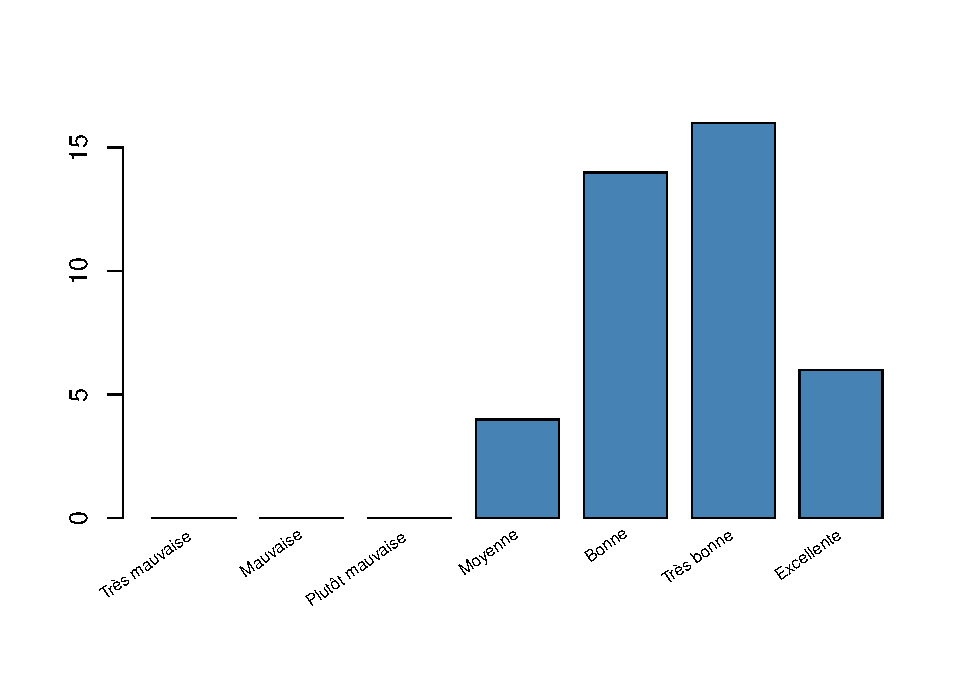
\includegraphics[width=0.75\textwidth]{rapport-finale_files/figure-latex/fig-1-1} 

}

\caption{Distribution des rivières selon leur niveau de pollution}\label{fig:fig-1}
\end{figure}

\hypertarget{la-relation-entre-hbi-et-la-richesse-spuxe9cifique}{%
\subsection{La relation entre HBI et la richesse
spécifique}\label{la-relation-entre-hbi-et-la-richesse-spuxe9cifique}}

Pour ce qui est de la relation entre l'HBI et la richesse spécifique
représentés dans la figure \protect\hyperlink{fig:fig-2}{2}, il y a une
corrélation négative de 0.1 entre le niveau de pollution (HBI) et la
richesse spécifique des espèces. Ainsi, il n'y a aucune relation
évidente entre les deux paramètres.

\begin{figure}[H]

{\centering 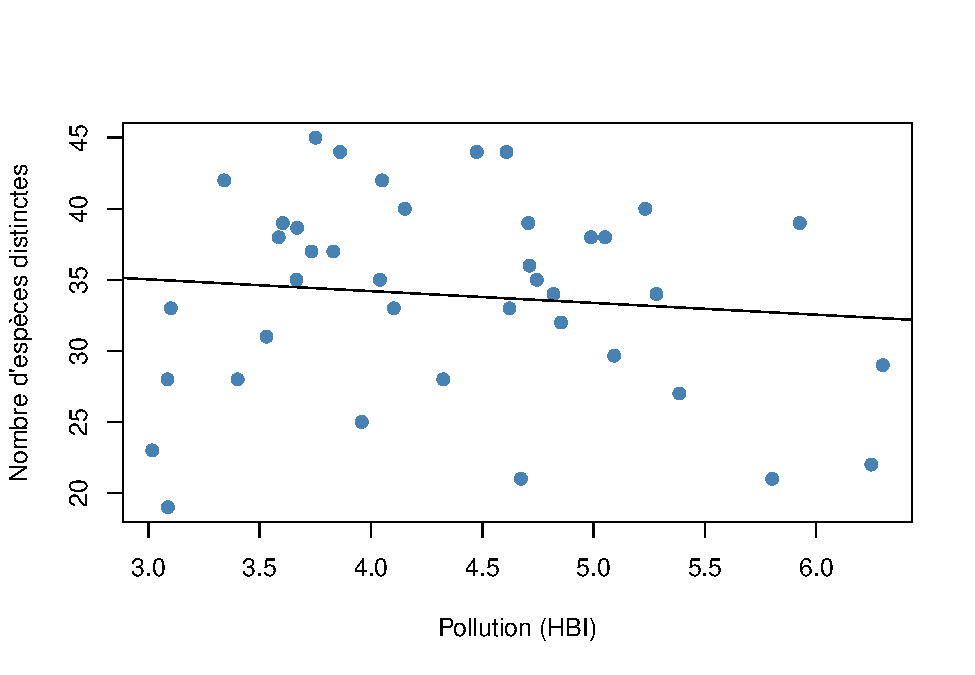
\includegraphics[width=0.7\textwidth]{rapport-finale_files/figure-latex/fig-2-1} 

}

\caption{Impact de la pollution sur la richesse spécifique des rivières}\label{fig:fig-2}
\end{figure}

\hypertarget{la-relation-entre-la-tempuxe9rature-et-la-richesse-spuxe9cifique}{%
\subsection{La relation entre la température et la richesse
spécifique}\label{la-relation-entre-la-tempuxe9rature-et-la-richesse-spuxe9cifique}}

En revanche, dans la figure \protect\hyperlink{fig:fig-3}{3}, la
température de l'eau montre une corrélation positive de 0.44 avec la
richesse spécifique des sites. Ainsi, plus la température est élevée,
plus il y a une grande diversité.

\begin{figure}[H]

{\centering 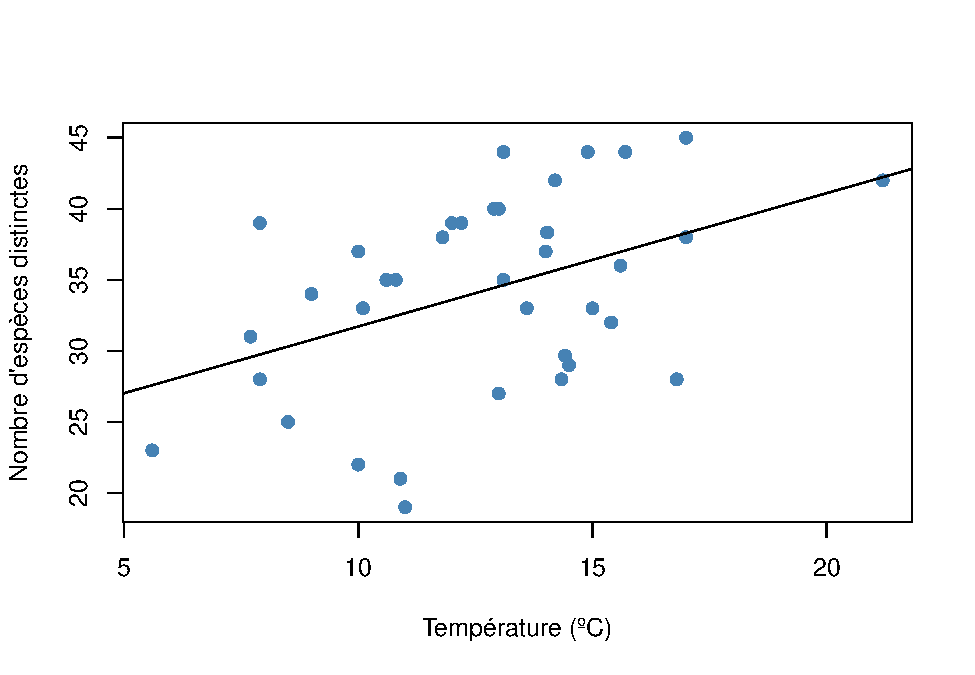
\includegraphics[width=0.7\textwidth]{rapport-finale_files/figure-latex/fig-3-1} 

}

\caption{Impact de la température des rivières sur leur richesse spécifique}\label{fig:fig-3}
\end{figure}

\hypertarget{discussion}{%
\section{Discussion}\label{discussion}}

Dans le but d'élucider les facteurs influençant la richesse spécifique
des rivières du Québec, deux paramètres clés ont été étudiés. Tout
d'abord, l'analyse de la corrélation entre le niveau de pollution,
évalué par l'indice biotique d'Hilsenhoff (HBI), et la richesse
spécifique des espèces aquatiques révèle une relation faible, presque
négligeable. Avec un coefficient négatif de 0.1, il semble que le niveau
de pollution ne joue pas un rôle déterminant majeur dans la diversité
des espèces dans ces environnements. D'autres variables non considérées
dans cette étude pourraient exercer une influence plus significative sur
la composition de ces communautés. De plus, les cours d'eau analysés
ayant tous un niveau de pollution relativement bas, cela pourrait
contribuer à diminuer l'impact de ce facteur.

En revanche, une corrélation positive notable de 0.44 entre la
température de l'eau et la richesse spécifique suggère une relation
beaucoup plus significative. Les sites où la température de l'eau est
plus élevée présentent une diversité d'espèces plus grande. En se fiant
à l'étude de \citet{bonacina_effects_2023}, la température a un impact
certain sur les macroinvertébrés. Chaque macroinvertébré a son étendue
de tolérance. Ainsi, on peut en conclure selon les données qu'un plus
grand nombre de taxons sont tolérants à des températures élevées qu'à
des températures plus basses.

Les variations observées et l'absence de corrélation forte suggèrent une
complexité dans les interactions entre la qualité de l'eau mesurée par
l'HBI, la température et la biodiversité des invertébrés benthiques. Des
facteurs supplémentaires, comme la présence de certaines espèces clés,
de la latitude et d'autres facteurs physiques, chimiques ou biologiques,
pourraient influencer ces résultats. En outre, l'effet de la température
sur la biodiversité des sites mérite une exploration plus détaillée,
afin de comprendre les mécanismes sous-jacents qui pourraient expliquer
la corrélation. Le changement de température a-t-il un impact plus
direct sur l'abondance de certains taxons en particulier, par exemple?

\hypertarget{conclusion}{%
\section{Conclusion}\label{conclusion}}

Cette étude a exploré les interactions complexes entre la qualité de
l'eau, mesurée par l'Indice biotique d'Hilsenhoff (HBI), la richesse
spécifique des invertébrés benthiques, ainsi que l'influence de la
température de l'eau sur ces paramètres. Nos résultats révèlent que,
contrairement aux attentes, il existe seulement une faible corrélation
entre l'HBI et la richesse spécifique. Ces constatations suggèrent que
d'autres facteurs environnementaux ou biotiques pourraient atténuer ou
amplifier l'impact des niveaux de pollution sur la biodiversité des
cours d'eau.

Par ailleurs, la température de l'eau a montré une corrélation plus
marquée avec la richesse spécifique, indiquant que les variations
thermiques pourraient jouer un rôle prépondérant dans la distribution
des communautés d'invertébrés benthiques. Ces découvertes mettent en
lumière la nécessité de prendre en compte une gamme plus large de
variables environnementales lors de l'évaluation de la santé des
écosystèmes aquatiques. D'autres études seront nécessaires pour
approfondir ce sujet.

\renewcommand\refname{Bibliographie}
\bibliography{bio500.bib}


\end{document}
